\documentclass[11pt]{article}       % The percent symbol in your code starts a comment.  The comment ends at the next linebreak.
\usepackage[english]{babel}         % Packages add functionality and style conventions to your documents. Don't edit this section!
\usepackage{fullpage}               % Eliminates wasted space
\usepackage[utf8]{inputenc}         % Necessary for character encoding
\usepackage{amsmath, amssymb,amsthm}% Required math packages
\usepackage{graphicx}               % For handling graphics
\usepackage[colorinlistoftodos]{todonotes}  % For the fancy "todo" stuff
\usepackage{hyperref}               % For clickable links in the final PDF
\usepackage{tikz}
\theoremstyle{definition}
\newtheorem{theorem}{Theorem}
\newtheorem{lemma}[theorem]{Lemma}
\newtheorem{prop}[theorem]{Proposition}
\newtheorem{claim}[theorem]{Claim}

\title{Complex Analysis -- Homework \#4}

\author{ Komissar, Feldman, Kallus }

\date{ Due Friday, February 12 }

\begin{document}
\pagecolor{black}
\color{white}
\maketitle

\noindent{\bf 1. } Claim: For all $z \in \mathbb C$, $\sqrt2|z| \geq |\text{Re}~z| + |\text{Im}~z|$.
\begin{proof}
    Let $z = x + iy \in \mathbb C$.
    \begin{align*}
    (|x|-|y|)^2 &\geq 0 \\
    |x|^2 + |y|^2 -2|xy| &\geq 0 \\
    |x|^2 + |y|^2 &\geq 2|xy| \\
    2(|x|^2 + |y|^2) &\geq |x|^2 + 2|xy| + |y|^2 \\
    \sqrt2|z| &\geq |x| + |y| \\
    \sqrt2|z| &\geq |\text{Re}~z| + |\text{Im}~z|.
    \end{align*}
\end{proof}

\bigskip
\noindent{\bf 2. } Exercise 5.5(a)

\centerline{
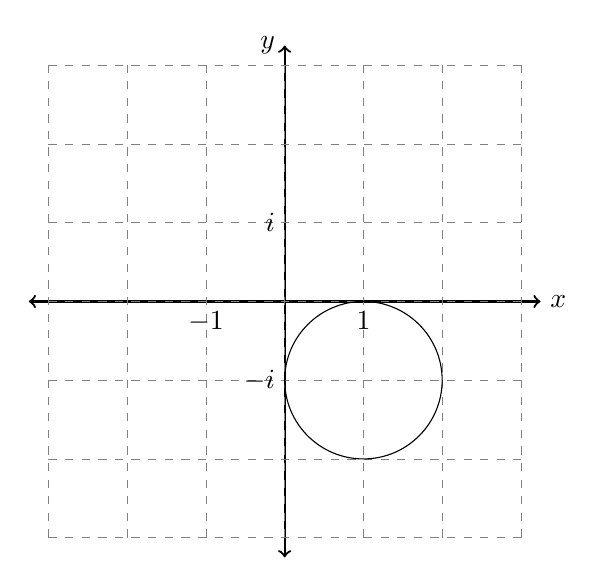
\begin{tikzpicture}[xscale=1, yscale=1]
    \draw [thick, <->] (0,3.25) -- (0,-3.25);
    \draw [thick, <->] (-3.25,0) -- (3.25,0);
    \draw [help lines] [dashed] (-3,-3) grid (3,3);
    \node [right] at (3.25,0) {$x$};
    \node [below ] at (1,0) {$1$};
    \node [below ] at (-1,0) {$-1$};
    \node [left] at (0,1) {$i$};
    \node [left] at (0,-1) {$-i$};
    \node [left] at (0,3.25) {$y$};
    \draw (1,-1) circle (1cm);
\end{tikzpicture}
}

\newpage
\noindent{\bf 3. Exercise 6.7 } Claim: For all $z \in \mathbb C$ such that $|z| \leq 1$, $|\text{Re}(2+\overline z + z^3)| \leq 4$.
\begin{proof}
    Let $z = a+bi$ be an element of $\mathbb C$ such that $|z| \leq 1$.
    Then,
    \begin{align*}
           |\text{Re}(2+\overline z + z^3)|
        &= |2 + \text{Re}(\overline z) + \text{Re}(z^3)| \\
        &= |2 + a + (a^3-3ab^2)| \\
        &= |2 + a(a^2 - 3b^2 + 1)|.
    \end{align*}
    Note that $0 \leq b^2 \leq 1$, since $a^2 + b^2 \leq 1$, and both $a^2$ and $b^2$ are positive.
    Similarly, $0 \leq a^2 \leq 1$.
    Thus, $-1 \leq a \leq 1$.
    Therefore, $-2 \leq a(a^2 - 3b^2 + 1) \leq 2$.
    Consequently, $|2 + a(a^2 - 3b^2 + 1)| \leq 4$.
    Therefore, $|\text{Re}(2+\overline z + z^3)| \leq 4$.
\end{proof}

\end{document}
